\chapter{Evaluation of NDT graph based SLAM}
In this chapter we will demonstrate functionality of our algorithm. We compare it with two well known \gls{SLAM} approaches implemented in \gls{ROS}. We also explain what parameters are needed to fully use potential of this algorithm. Whole experiment is conducted by running prerecorded data files from PR2 robot operating in \gls{MIT} Sata Center \cite{MITDataset}. We have selected this dataset because laser scanner provides sufficient number of points to produce \gls{NDT} fields with normal distribution. It is also recorded in form of "bag file" which is standard format in \gls{ROS}. It offers very challenging situations for robust testing. It is not uncommon that algorithms fail on many of recorded data sets. The problem is even more difficult when using only 2D laser data information.

\section {MIT dataset details}
This dataset offers fine laser data with 1130 points per scan. The sensor's field of view is 260 degrees.The 2D laser scans have maximum range of 60 m with publishing frequency around 20 Hz. The dataset was recorded on multiple floors of the Sata Center. This means that robot enters an elevator and is transported to different floors. Therefore, we have selected only data sets which stay on the same floor. Our experiments were conducted only on the second floor because it has information about ground truth.

We have selected two datasets which we think showcase well possibilities of this algorithm. First dataset runs in small loop inside of one room. This is challenging because robot needs to correct its position multiple time. It is also computationally difficult for loop closure mechanism. In every iteration it needs to compare its position with all previous measured data. Iterative movement at the same place can also demonstrate robustness of incremental scan matcher again any shift caused by registration error.

Second dataset starts in the long corridor and moves in direction towards room from the first selected dataset. It again do multiple loops and then it moves through corridor to new room. It maps this room and returns through the same corridor. In this type of setup odometry information or incremental scan matching can accumulate error over long corridor and last room, which should be visible on the returning trip. This tests loop closure mechanism over long distance.

In the figure \ref{fig:ground_truth} is a map of used datasets built with \gls{NDT-OM} with transformation between scan originating in ground truth measurements provided with dataset. 

\begin{figure}
	\centering
	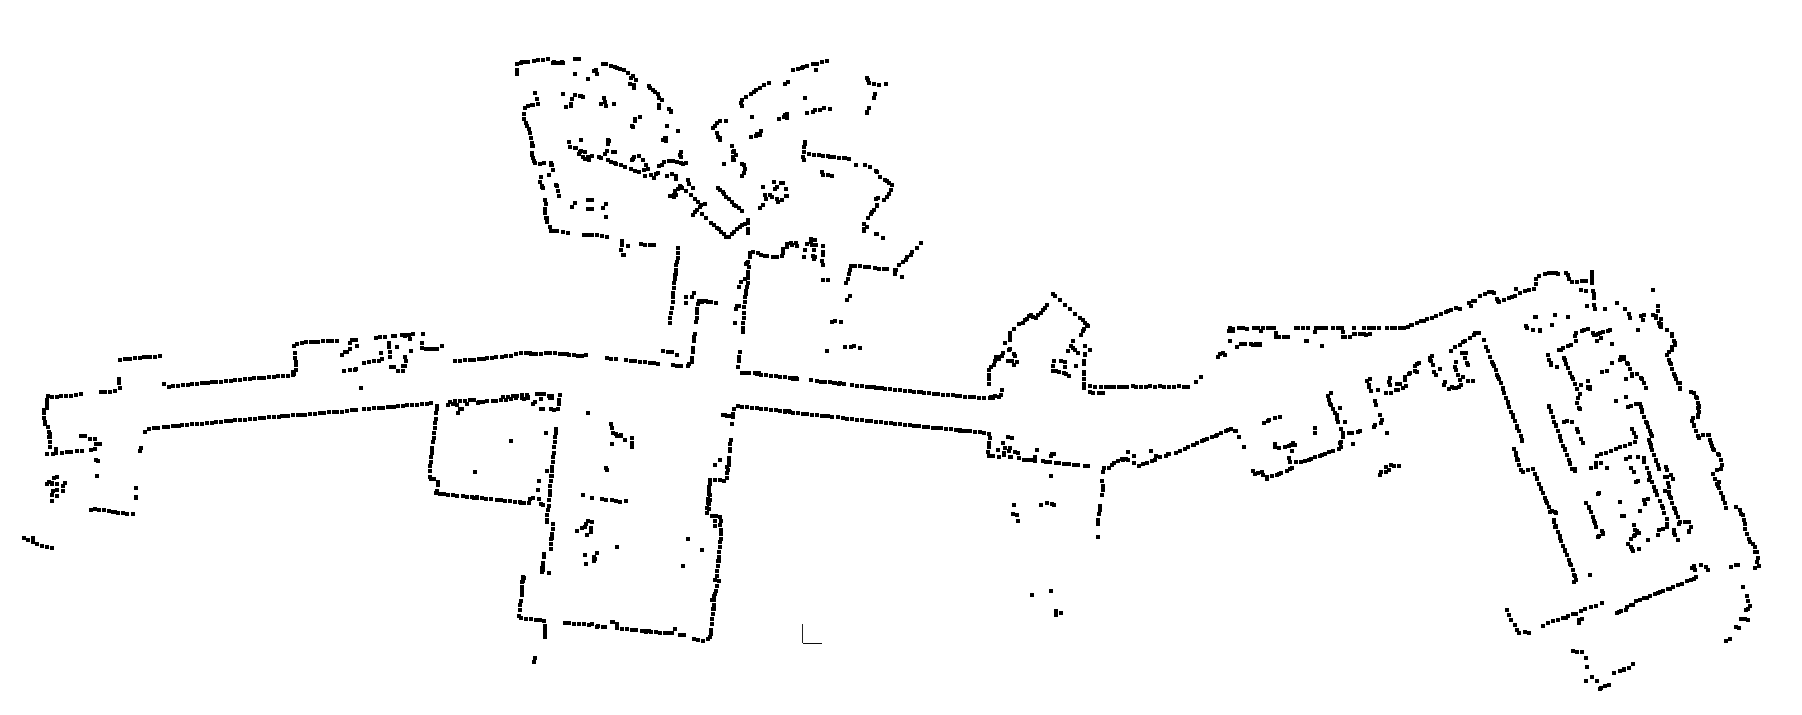
\includegraphics[width=140mm]{../img/ground_truth.png}
	\caption{The \gls{NDT} map generated out of selected datasets with use of ground truth odometry information.}\label{fig:ground_truth}
\end{figure}
  
\section{ROS SLAM algorithm overview}
\subsection{The Gmapping}
The Gmapping proposed by \cite{gmapping} is the popular \gls{SLAM} algorithm in \gls{ROS}. It is based on Rao-Blackwellized particle filters. In this algorithm each particle is carrying representation of the map. In this set up number of particles is rapidly increasing memory requirements. For this reason authors used not only odometry to estimate robot movement but also the most recent measurements. This reduces number of samples by providing better estimate of robot's movement. The Gmapping was used in dozens of projects in ROS. It is usually first \gls{SLAM} used by every novice user in \gls{ROS}. It is well documented and tested. Output representation is in form of occupancy grid with fine resolution 0.05m. 
\subsection{The Hector SLAM}
The Hector \gls{SLAM}  proposed by \cite{Hector} uses fast and robust scan matching to estimate robots movement and build map. The algorithm also do not use any odometry which makes it ideal for aerial robots. Registration is done by optimalization of laser end points with map built in previous iterations. Registration equation is solved using a Gaussian-Newton minimization method. This process returns transformation between laser endpoints with resulting map. This method may converge into local minimum. Authors prevent this by using multiple grids each with coarser resolution. This method operate on top of occupancy grid with fine resolution around 0.05m.

In comparison to our method it is very similar to our front end odometry estimator. Our method of running window uses fast incremental scan matching. It also uses several layers to avoid local minimum. The biggest difference is used underling map model. In our algorithm we use map with coarse cell size 0.25m with \gls{PDF} inside. In addition, we also have loop closure engine with pose graph which should resolve more difficult localization errors.

\section{NDT-GraphSLAM evaluation}
In all our experiments we have used our \gls{SLAM} algorithms as was described in section \ref{sec:Sys_arch}. We have decided to set moving window size to max range of the sensor which is 60 m in our dataset. We have also set fixed values for radius search for loop detection to 20m. We selected this value so we can test as many loop closures as possible. During our mapping and localization test we also record all loop closure measurements. These are saved to the disk as point cloud file (.pcd). We also save results of loop closure registration with resulting score for evaluation of loop closure algorithm based on changing parameters. Files from experiments are available in an attachment of this work. Initial value for loop closure registration threshold was set to 0.6. Every loop registration with score higher than this value will be inserted into the graph as loop closure edge. 

Output from our method is in point clouds. Each point represents position of mean value inside of the cell. Resolution of this map is same as for all \gls{NDT} grids (0.25m). Our representation is different in  comparison to output methods of Gmapping and hector mapping which use occupancy map. Representation of the output map does not change characteristics of reconstructed maps. It is important that map has correct shape. It is also important that empty places like hallways or centers of the rooms stay unoccupied with as little noise as possible. Result should not include any phantom walls. These are walls present on the map but they do not exist in reality. They are usually caused by wrong pose estimation. In our representation we also output pose graph visualization which is only for debugging and demonstration purposes. 

\subsection{NDT frame generation frequency}
In this experiment we wanted to test what is optimal euclidean distance between two consecutive \gls{NDT} frames. We use same representation of frames as mentioned in section \ref{sec:NDT_frame}. Based on design of the system this parameter should influence quality loop closure detection and evaluation. In order to test this parameter we have decided to test it on second dataset with distances 1m 2m and 4 meters.

One meter range has generated frame every 1 meter of robot's trajectory. This has created high amount of nodes with small map representation of environment inside. For mapping purposes this created nice map because there was small odometry error inside of frame. Error may be caused by wrong odometry estimate from moving window. This can be observed in the first picture of figure \ref{fig:frame_freq}. Its also important to note that it has generated the biggest amount of loop closure edges. This mainly thanks to fact that it is easier for two frames get high overlapping score from robust D2D if they have no errors inside. On the other hand it is more probable that these scans will have problems with ambiguities. This has happened in total 4 times in the second dataset with registration threshold set to 0.6.

The second variant with two meters long distance between frames offered optimal results. It has generated fewer nodes than the first variant. Loop closure edges added to the graph were able to repair errors from odometry estimation and still keep same quality of map.

The third variant failed to find loop closures. Every frame had data with heavy noise inside. This caused that non of the loop closing tests received score more than 0.1.

Based on these results we have decided to use fixed distance of 2 meters between two frames in the next tests.


\begin{figure}
	\centering
	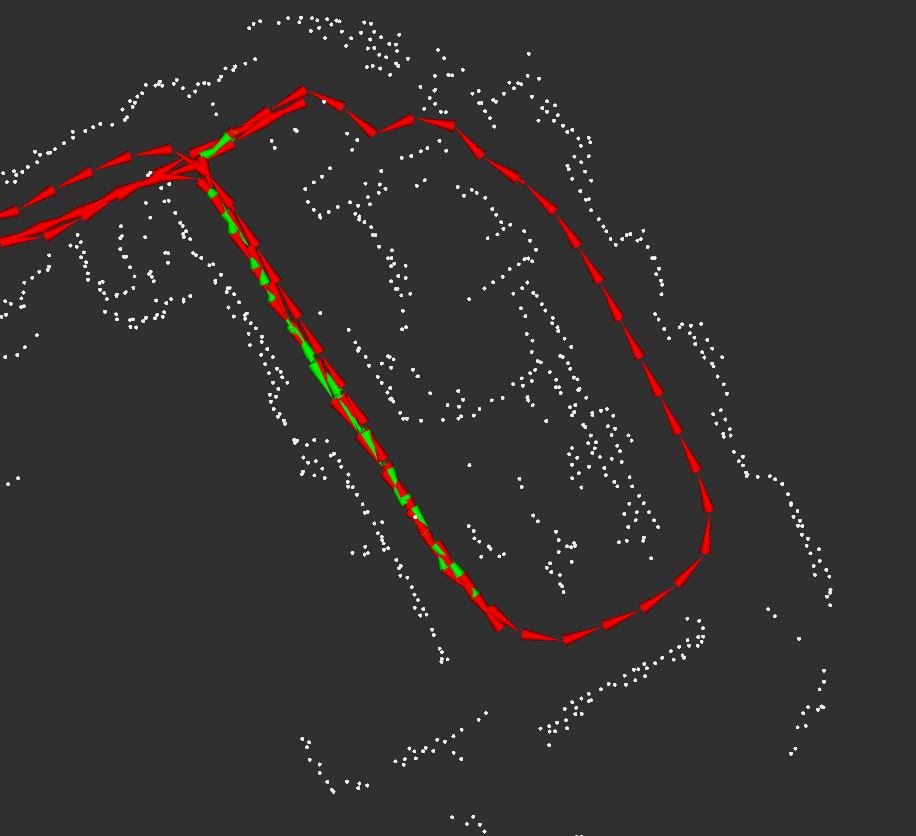
\includegraphics[width=70mm]{../img/gen_len1.png}
		\vspace{0.1cm}
	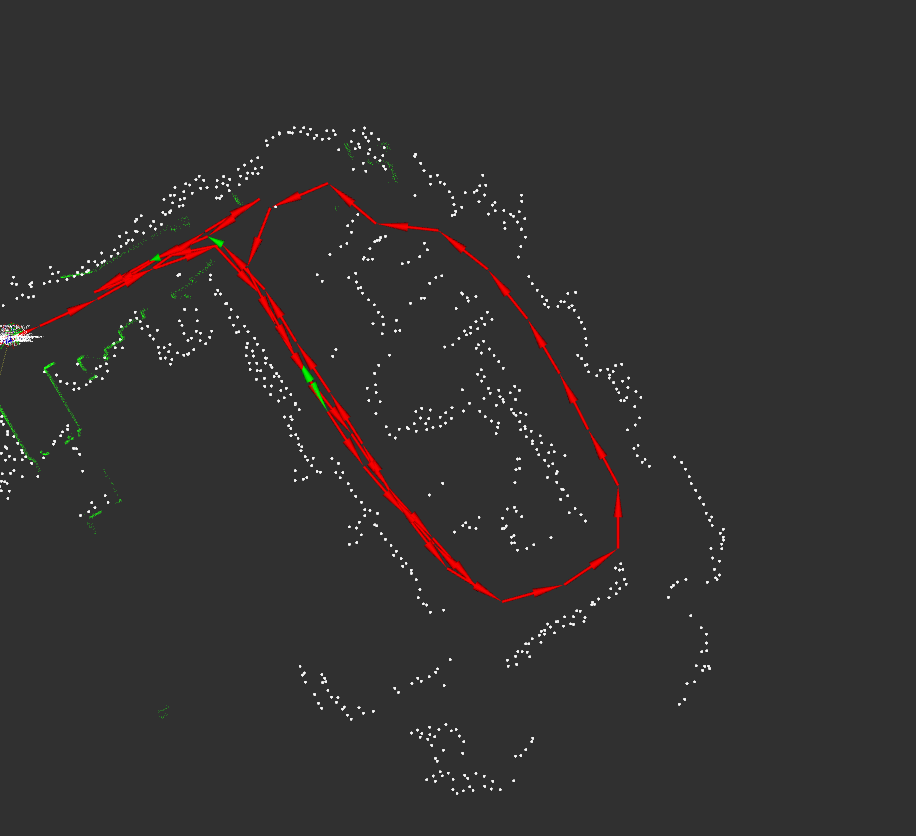
\includegraphics[width=70mm]{../img/gen_len2.png}
	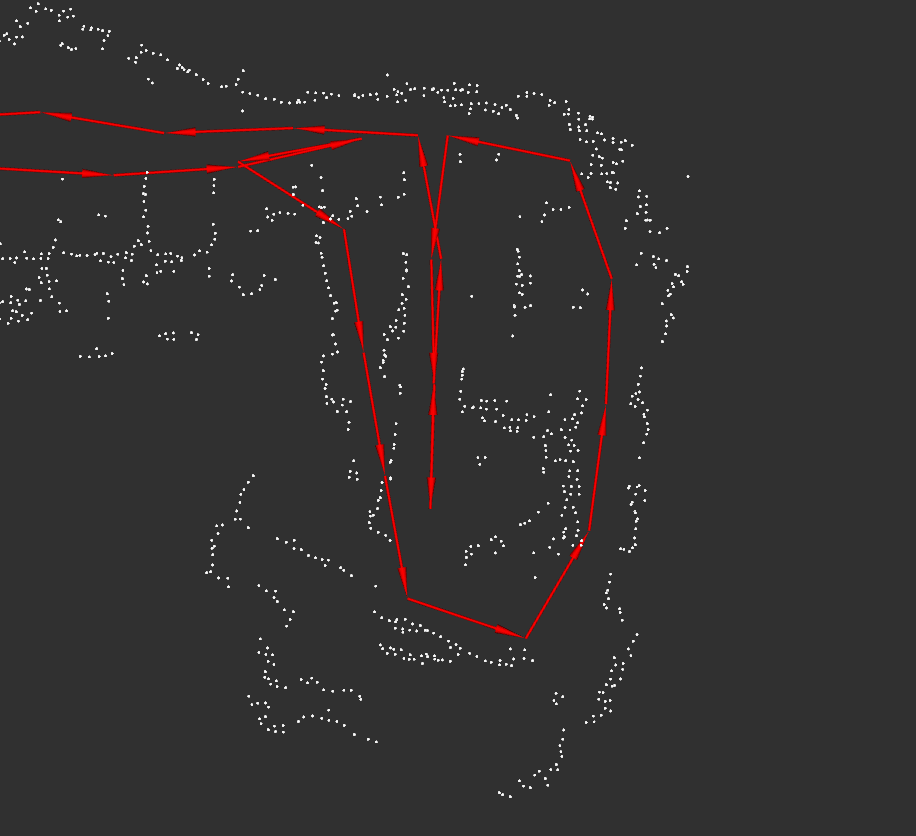
\includegraphics[width=70mm]{../img/gen_len4.png}
	\caption{Comparison of effect of different frequency of frame creation. From left pictures of 1m, 2m and 4 meter distance between frames. Red arrows represent odometry edges, green edges are loop closure edges, white dots represent point cloud of means from each cell.}\label{fig:frame_freq}
\end{figure}
\subsection {Robust D2D score threshold}
In a previous section we have use fixed registration threshold to value 0.6. In this section we will test if this is really optimal value. This test is executed by first setting threshold to value 0.6. Then running second dataset. All measurement data received from all loop closure registration are sorted based on score value into groups. The first group  has score range from 0.4 to 0.49. The second group from 0.5 to 0.59. The third group starts at 0.6 and ends in 0.69. Last group include all loop closures with higher value. We will look at number of edges in each category which are have wrong alignment. These edges are usually created on failure of algorithm to register correctly frames. The other reason might be ambiguity in the environment. We want to minimize number of incorrect edges in our graph. Result of this experiment is in \ref{fig:robust_matcher_res}.

Based on result we can conclude that algorithm is able to securely identify valid loop closure on this dataset if score is above 0.6. One error in this category was caused by ambiguity in long corridor. This error is not possible to correct by usual registration algorithms. \ref{sec:reg_alg} Other two categories equally include more errors than correct results. Errors can be divided into two types. Some incorrect registrations are caused by matching unrelated places. These places are different but it is possible to match them in a way which yields good score. Score assigned by matcher is usually lower than 0.55. Some errors are also registration failures. In this type of error mostly depends on the structure ambiguity inside of the frame. This happens if two frames include same area but each has dominant number of cells mapping different feature of environment. This ambiguity makes robust estimator connect these two parts. This increases score in these likely part to higher levels. On the other hand parts of the frames not matching each other lower the score. As a result score of these errors ranges is in whole range from 0.4 up to 0.6.

Based on this experiment we can set to 0.6 or higher and get enough high quality loop closures to fully correct graph.    


\begin{figure}
 \centering
  \begin{tabular}{ | c | c | c | c | }
    \hline
    &correct&error&total\\ \hline
    [0.7,1] & 21 & 0& 21\\ \hline
    [0.6, 0.7) & 33 & 1& 34\\ \hline
    [0.5, 0.6)] & 18 & 26& 44\\ \hline
    [0.4, 0.5)]& 13 & 28& 31\\
    \hline
  \end{tabular}
	\caption{Number of correct and incorrect registrations in score groups}  \label{fig:robust_matcher_res}
\end{figure} 

%\begin{figure}
%	\centering
%	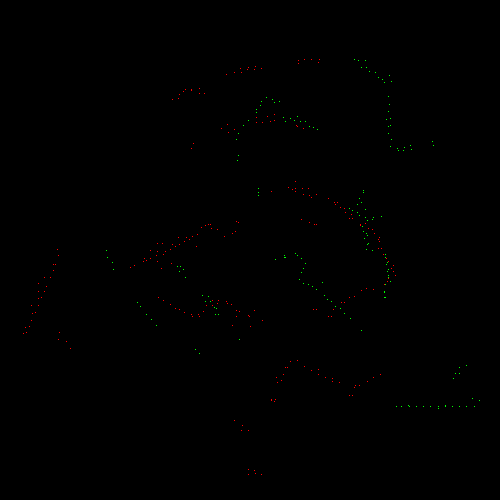
\includegraphics[width=70mm]{../img/robust_error1.png}
%		\vspace{0.1cm}
%	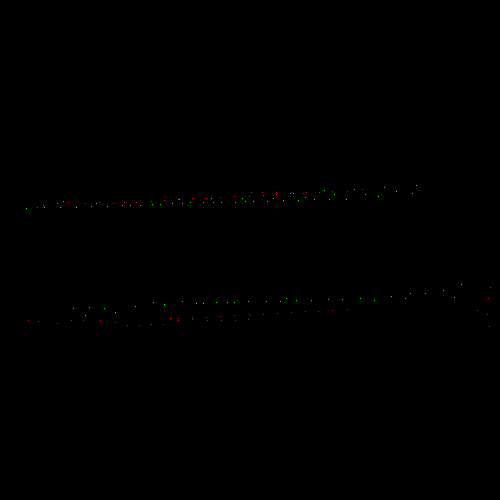
\includegraphics[width=70mm]{../img/robust_error2.png}
%	\caption{Comparison of effect of different frequency of frame creation. From left pictures of 1m, 2m and 4 meter distance between frames. Red arrows represent odometry edges, green edges are loop closure edges, white dost represent final map representation in form of point cloud of means}\label{fig:frame_freq}
%\end{figure}
%\subsection{Performance}
%Performance of this algorithm is important measure. If it is supposed to run in online it needs to be fast enough. In this experiment we have tested individual parts of algorithm which takes up most of the time. First we need to be able to incrementally register incoming scans. This make requirements on speed of incremental scan matcher. Secondly we need to test as many loop closures as possible. Testing loop closures is the most time demanding operation in graph processing. In our test environment we have run each registration algorithm on the second corridor dataset. This meant registering total of 10000 measurements. 
\subsection{Iterative mapping of room}
\begin{figure}
	\centering
	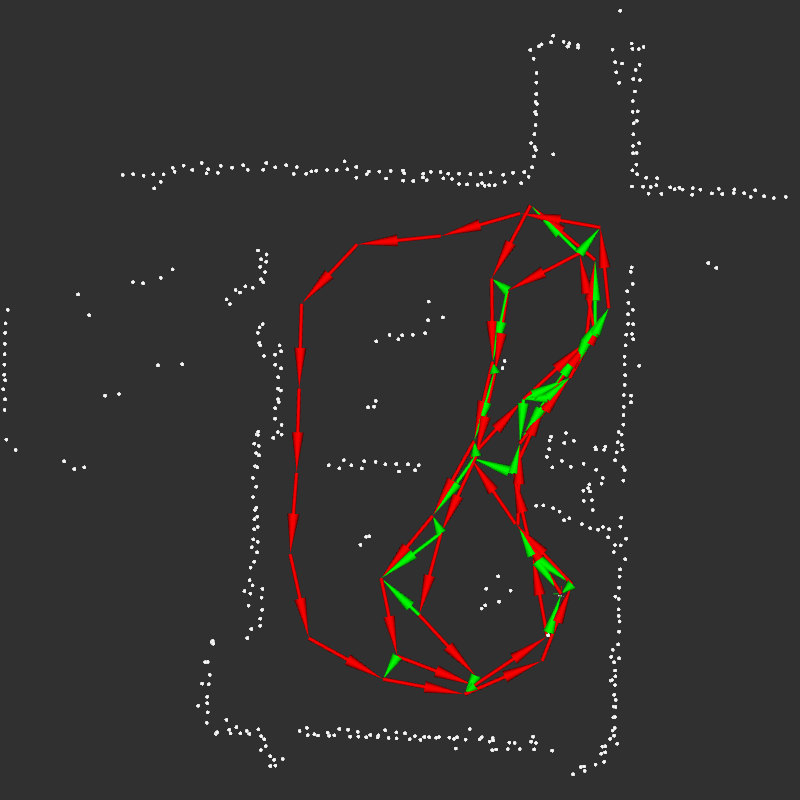
\includegraphics[width=70mm]{../img/room_ndt.png}
		\vspace{0.1cm}
	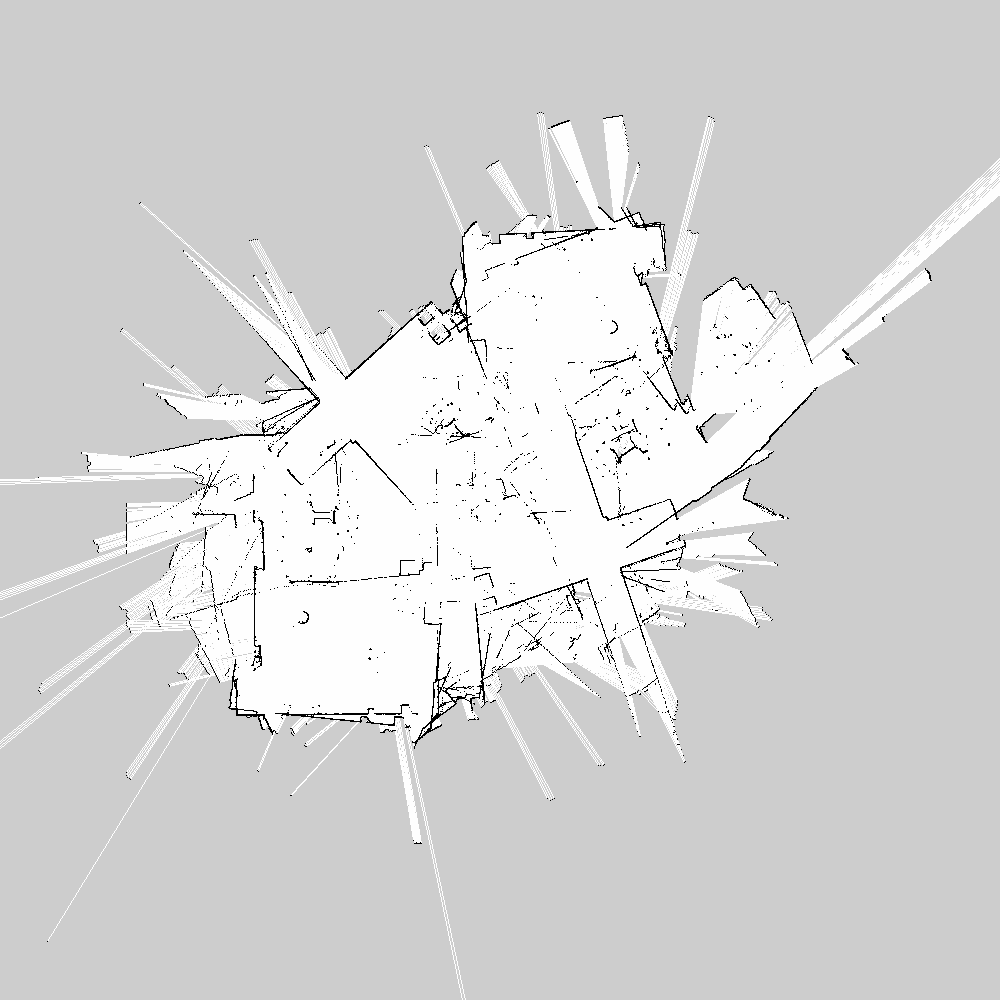
\includegraphics[width=70mm]{../img/room_hector.png}
	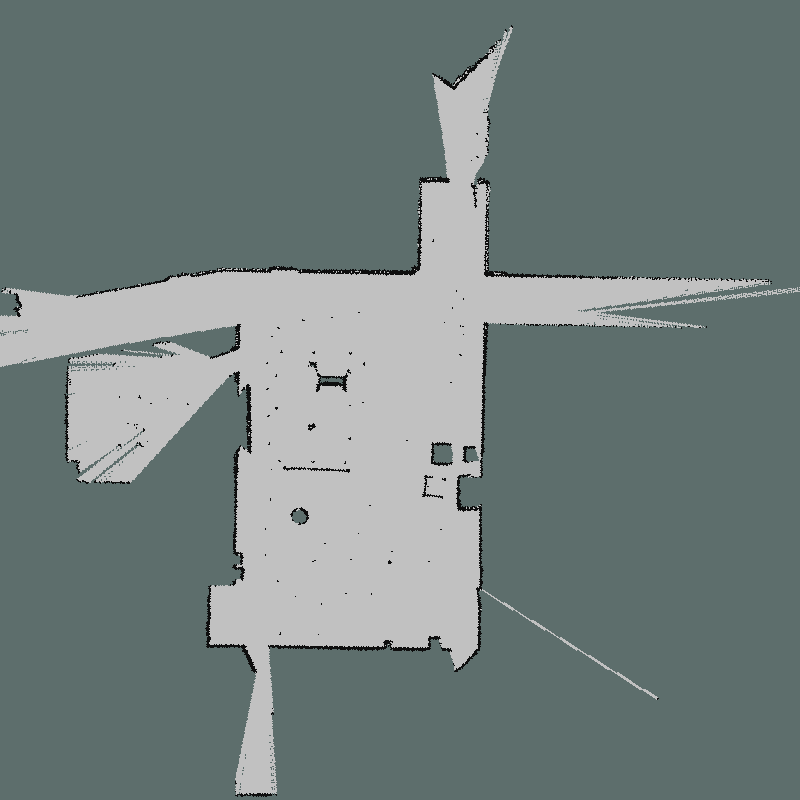
\includegraphics[width=70mm]{../img/room_gmapping.png}
	
	\caption{Map of the room mapped by our NDT aproach, Hector mapper and Gmapping. Visualization of our aproach includes visualization of pose graph with red odometric edges and green loop closure edges. White spots represent means of each cell's  normal distribution.}\label{fig:room_res}
\end{figure}
This dataset represents single room. In order to fully map it robot moved multiple time around the room. Every movement carries some error. It is necessary to correctly align consecutive scans. This well demonstrates coordination of moving window with loop closure mechanism. Whole room has fitted inside the moving window and registration provided robust transformation for \gls{NDT} frame building process. Loop closures were correctly identified all above threshold 0.6. Distance between frames is 2m as discussed previously. Map is compact and without any defects.

Hector mapping has not converged into correct output. It was not able to cope with rotations of the robot in this dataset. We have also tested slowing down dataset with rate 0.6. This has not helped to hector recover correct data.

The Gmapping offers  solution with similar quality to our result. 

\newpage
\subsection{Long corridors}
Long corridor dataset was selected because it maps two main rooms plus it adds mapping of top part of the map. This part with its irregular shapes proven to be very difficult mostly for hector mapping. It has failed mapping process as you can see on the middle image in figure \ref{fig:full_res}. The Gmapping algorithm offered accurate result.

Our approach has recovered main shape of the map correctly. Small difference is in noisiness of the walls. Our algorithm has higher noise. Main reason is different mapping model. The Gmapping and hector mapping are both using extremely fine map with resolution 0.05m. Our approach is using coarser 0.25m grid for visualization. Our map is coarser but still covers and represent free space correctly without noise. Coarser grid has also advantage in path planning or ray-tracing which is faster. Finer grids often needs to be converted into lower resolutions to work with them efficiently.

Second difference is length of the corridors. Our approach has shortened length of corridors. This happened because of data ambiguity. Robot passing through these corridors do not see the end of hall. This makes him observe only two straight walls on the right and on the left. Without prior information about robot movement, this is correctly understood as robot standing still without movement. The way our algorithm deals with this type of errors is by closing loop closure when returning on the same place through different path. In this case robot used same trajectory, which lead to same error only in the opposite direction. The only other solution how to sove this problem is to integrate movement of robot into moving window incremental scan matching. Resulting cooridor than look like in figure \ref{fig:corridor}. 
\begin{figure}
	\centering
	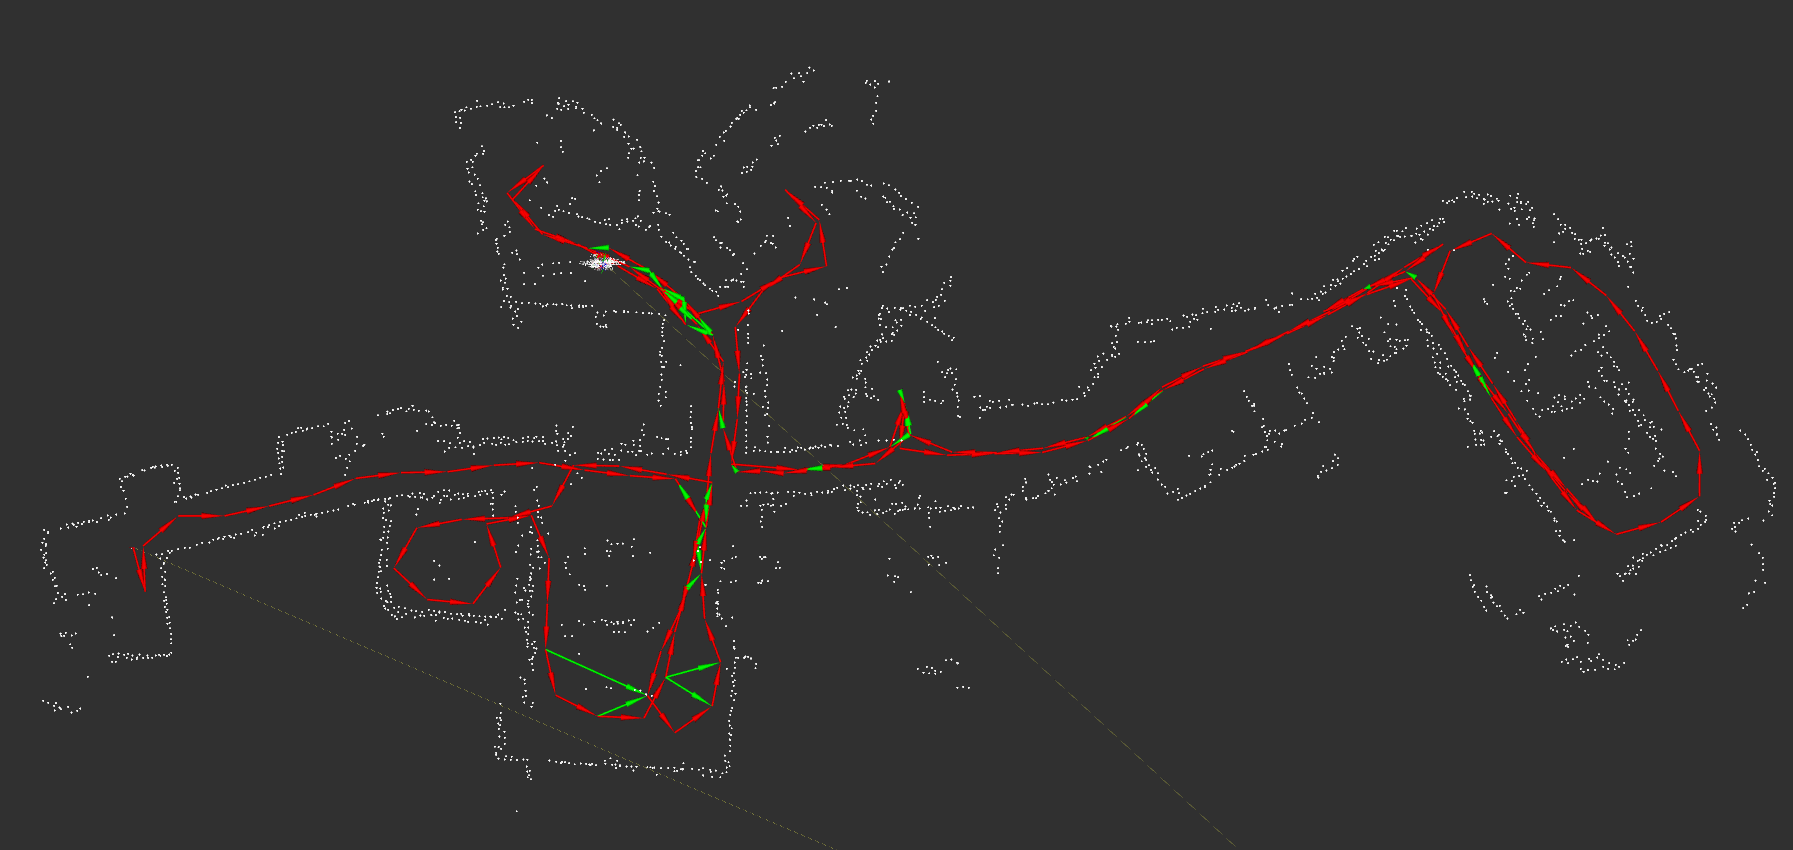
\includegraphics[width=140mm]{../img/full_ndt.png}
	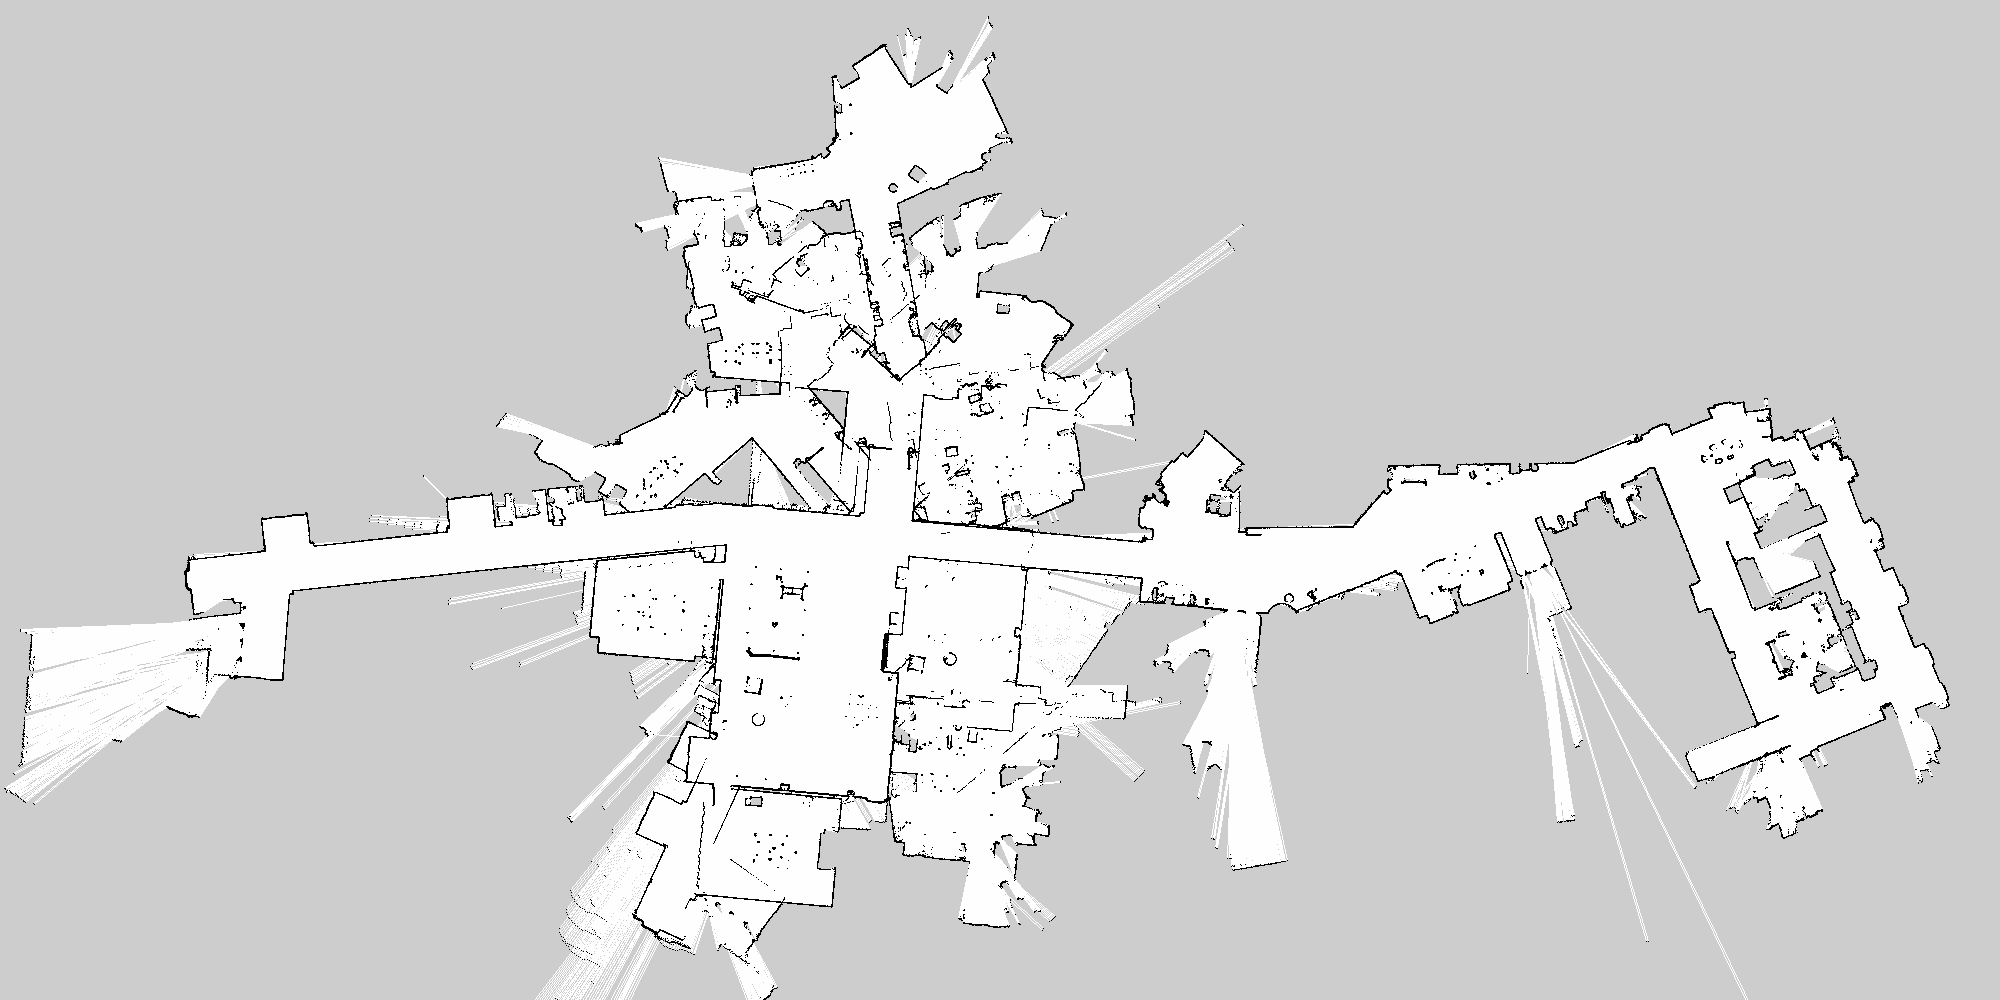
\includegraphics[width=140mm]{../img/full_hector.png}
	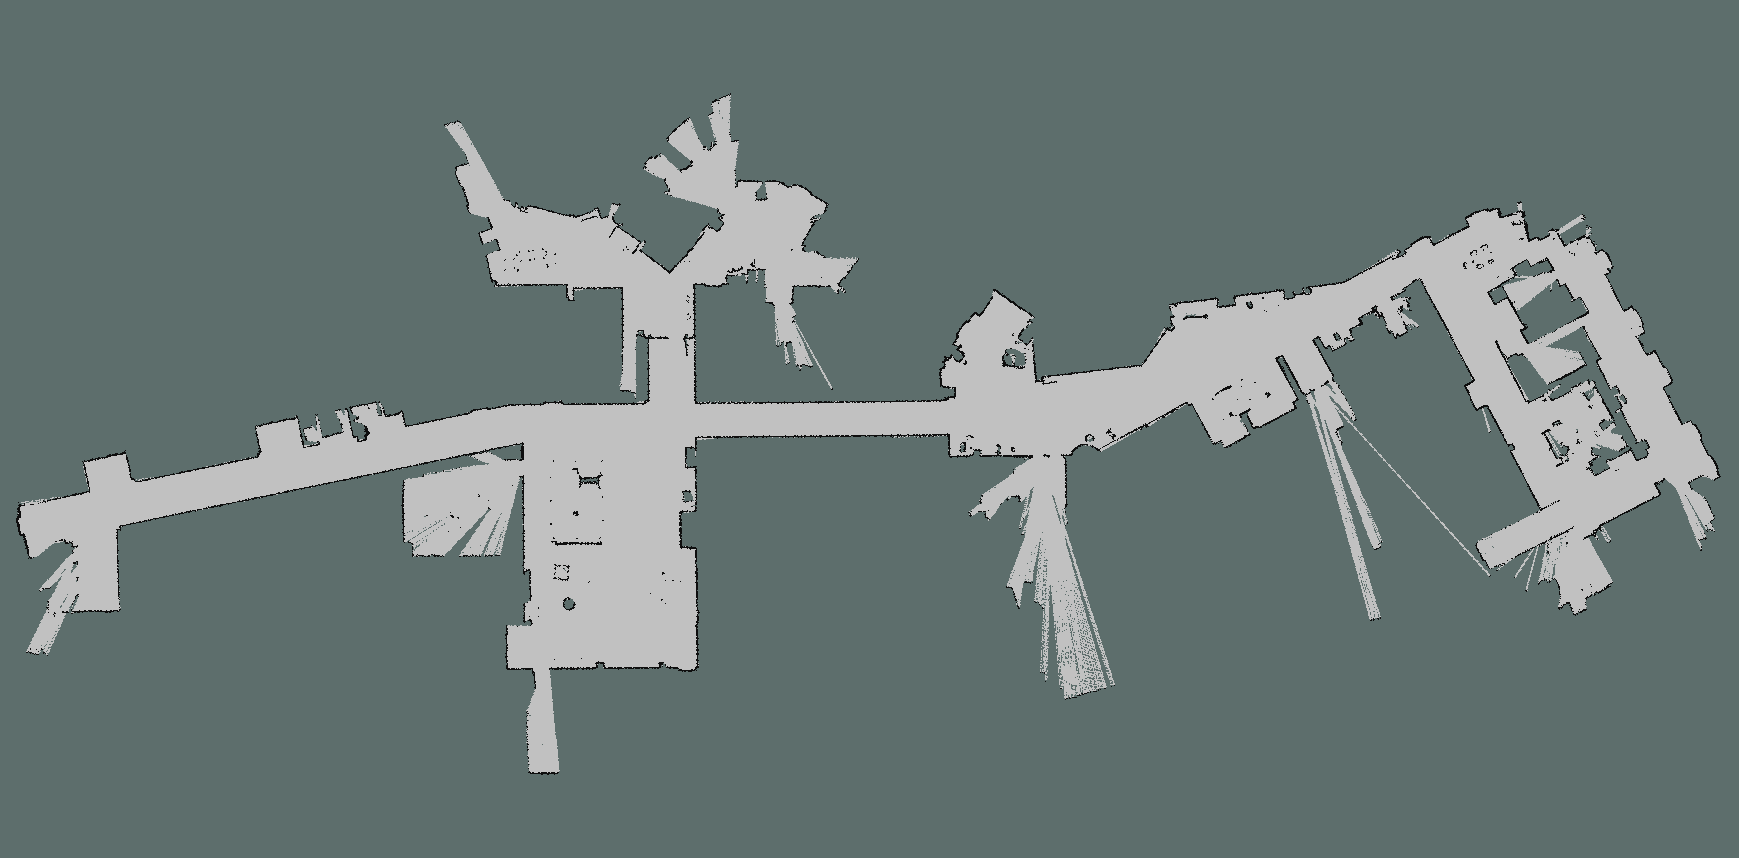
\includegraphics[width=140mm]{../img/full_gmapping.png}
	
	\caption{Map of the corridors mapped by our \gls{NDT} approach, hector mapper and Gmapping. Visualization of our approach includes visualization of pose graph with red odometric edges and green loop closure edges. White spots represent means of each cell's  normal distribution.}\label{fig:full_res}
\end{figure}

\begin{figure}
	\centering
	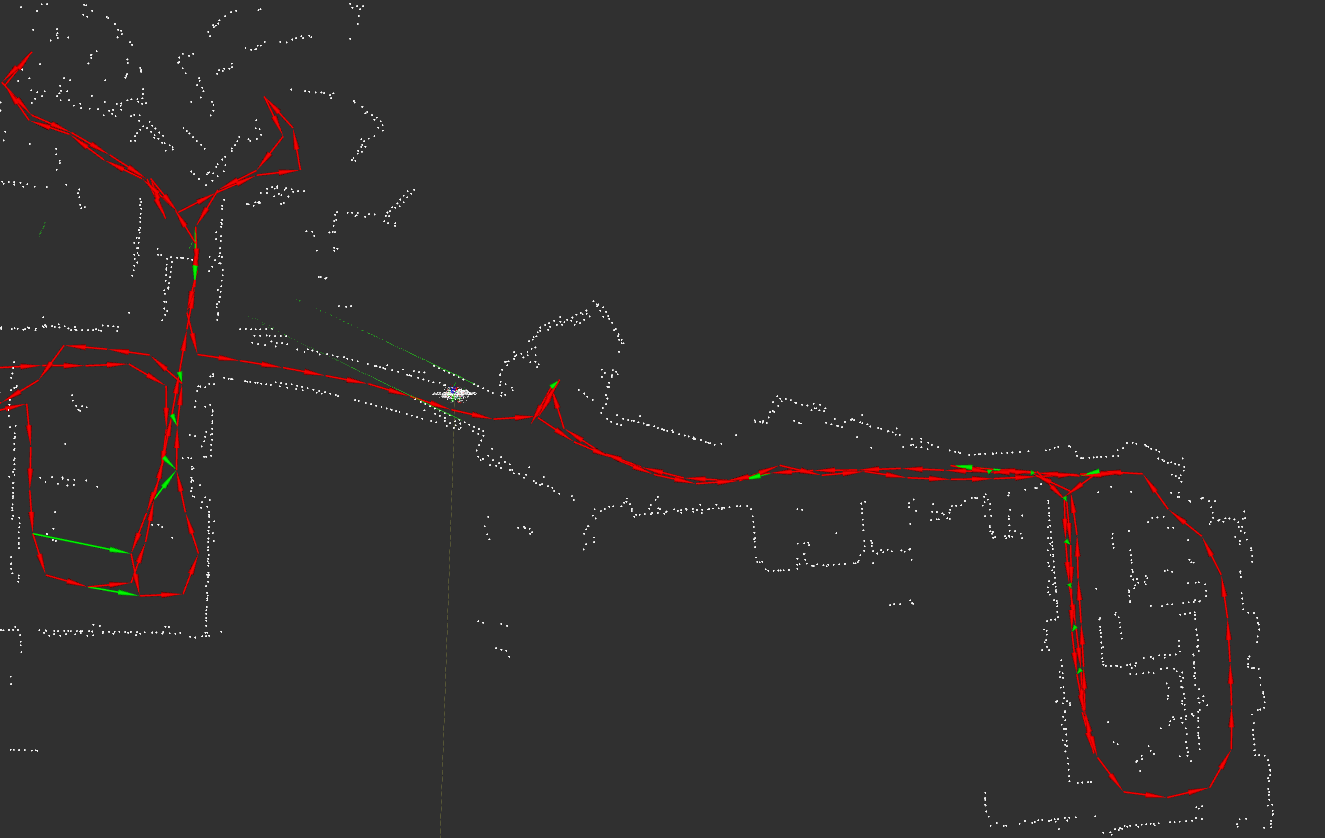
\includegraphics[width=140mm]{../img/coridor.png}
	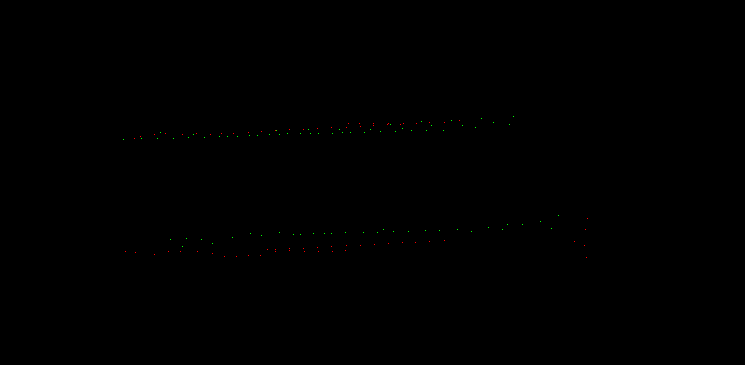
\includegraphics[width=140mm]{../img/coridor2.png}

	\caption{Top picture shows portion of map with corridor when incremental scan matcher may use initial guess from odometry. Bottom picture shows ambiguous registration in corridor area.}\label{fig:corridor}
\end{figure}